\documentclass{boi2014}

\usepackage{enumitem}
\usepackage{wrapfig}
\usepackage{mathtools}
\usepackage{tikz}

\renewcommand{\DayNum}{1}
\renewcommand{\TaskCode}{coprobber}
\renewcommand{\TaskName}{Cop and Robber}
\renewcommand{\TaskVersion}{1.3}

\renewcommand{\labelitemii}{$\circ$}
\newcommand{\constant}[1]{{\tt #1}}

\begin{document}
    \begin{wrapfigure}[8]{r}{6cm}
        \vspace{-24pt}
		\includegraphics[width=6cm]{\TaskCode.jpeg}
	\end{wrapfigure}

    In the city of Bytemore crime level is hitting an all--time high.
    Among other misdemeanours, robberies are happening every day.
    And when the crime is committed, it is always up to a lone patrolling
    police officer to chase down the robber through the narrow alleys
    that connect street corners (commonly referred to simply as
    \emph{corners}). Unfortunately, more often than not, robbers escape
    their pursuers, because they know the city much better than
    the police.

    The Bytemore City Police Department (BCPD) is organising a summit
    to reduce crime. One of the initiatives is to use computer aid when
    pursuing the robbers. For this purpose, the BCPD has made a precise
    map of the city. Now they need computer software to find chasing
    strategies.

    The pursuit problem of one officer chasing one robber is modelled
    as follows:
    \begin{enumerate}
        \item The police officer chooses a corner on which to patrol.
        \item The robber then chooses a corner for the robbery
            (he knows where the officer is). From this moment on it
            is always assumed that both the officer and the robber
            know where each other is.
        \item The police officer's move consists of him moving to a
            neighbouring corner (i.e. one that is connected to the
            current one by an alley) or waiting (i.e. not moving).
        \item The robber's move consists of him moving to a neighbouring
            corner. Note that, unlike the police, robbers cannot wait.
            It is in their instinct to keep running.
        \item The police officer and the robber keep making moves one after
        another (starting with the officer) until one of the following
        happens:
        \begin{enumerate}
            \item situation repeats itself (situation is defined
                by the positions of both agents and the side whose turn
                it is to move next). This corresponds to the robber being
                able to avoid the police officer indefinitely, so the
                robber escapes;
            \item the police officer and the robber meet on the same corner
                after a move of either of them. In this case the police officer
                catches the robber.
        \end{enumerate}
    \end{enumerate}

    \Task
    You have to write a program which, given the map of the city,
    would determine whether catching the robber is possible, and if it is,
    would catch him by making moves on behalf of the police officer.

    Your program must assume that the robber moves optimally.

    \Implementation
    You need to implement two functions:
    \begin{itemize}
        \item \method{start(N, A)} which takes the following parameters:
            \begin{itemize}
                \item $N$ --- the number of corners (corners are labelled
                    from $0$ to $N-1$);
                \item $A$ --- a two--dimensional array that describes the
                    alleys: for $0 \le i, j \le N-1$,
                    $$
                        A[i, j] \text{ is }
                        \begin{dcases*}
                            \texttt{false} & if $i$ and $j$ are not joined by any alley
                                \\
                            \texttt{true} & if $i$ and $j$ are joined by an alley
                        \end{dcases*}
                    $$
                    All alleys will be bidirectional (i.e. $A[i, j] = A[j, i]$
                    for all values of $i$ and $j$) and there will be no alleys
                    connecting a corner to itself (i.e.  $A[i, i]$ will be
                    \texttt{false} for all values of $i$).  Also, you may assume
                    that it will always be possible to reach any corner from any
                    other corner by moving along the alleys.
            \end{itemize}

        If it is possible to catch the robber on the map described
        by the parameters, function \method{start} should return the
        label of the corner on which the police officer chooses to patrol.
        Otherwise, it should return $-1$.

        \item \method{nextMove(R)} which takes as a
            parameter the label $R$ of the current corner of the robber
            and must return the label of the corner where the officer
            will be after his move.
    \end{itemize}

    Function \method{start} will be called exactly once before any
    calls to \method{nextMove} are made. If \method{start} returns
    $-1$, then \method{nextMove} will not be called. Otherwise,
    \method{nextMove} will be called repeatedly until the pursuit ends.
    More precisely, the program will terminate as soon as one of the
    following happens:
    \begin{itemize}
        \item \method{nextMove} returns an invalid move;
        \item the situation repeats itself;
        \item the robber is caught.
    \end{itemize}

    \Example
    \begin{wrapfigure}[4]{r}{2cm}
        \vspace{-0.5cm}
        \centering
        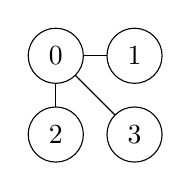
\begin{tikzpicture}
        \draw (0,1) -- (0,0);
        \draw (0,1) -- (1,0);
        \draw (0,1) -- (1,1);
        \foreach \x in {0,1} \foreach \y in {0,1}
            \draw (\x,\y) node[circle,draw,fill=white,inner sep=0,minimum size=0.7cm] {\pgfmathparse{int(2-2*\y+\x)}\pgfmathresult};
        \end{tikzpicture}
    \end{wrapfigure}
    Let's take a look at the example illustrated on the right. In this case any
    corner is a good starting position for the police officer. If he starts in the
    corner 0, he can wait in his first move and the robber will run into him.
    On the other hand, if he starts on any other corner, he can wait until the
    robber moves to corner 0, and then move there.
    
    Here's how a sample session could look like:

    \begin{tabular}{|l|c|}
        \hline
            {\bf Function call} & {\bf Returns} \\
        \hline
            \method{start(4, [[0, 1, 1, 1], [1, 0, 0, 0], [1, 0, 0, 0], [1, 0, 0, 0]])} &
            \constant{3} \\
        \hline
            \method{nextMove(1)} & \constant{3} \\
        \hline
            \method{nextMove(0)} & \constant{0} \\
        \hline
    \end{tabular}

    Note: in the call to \method{start} above \constant{0} denotes
    \constant{false} and \constant{1} denotes \constant{true} for brevity.

    \Scoring
    
    \begin{description}
        \item[Subtask 1 (16 points):] $2 \le N \le 500$.
        Each pair of corners will be connected by exactly one path of alleys.
        \item[Subtask 2 (14 points):] $2 \le N \le 500$. The network of corners
        and alleys will form a grid-shaped structure. The grid will have at
        least two rows and columns and the street corner labelling will follow
        the pattern illustrated below.
        \begin{figure}[h!]
           \centering
           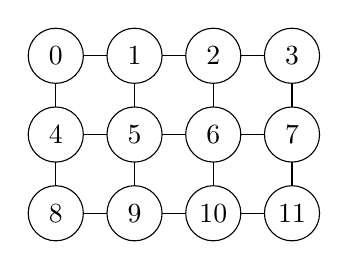
\begin{tikzpicture}
            \draw (0,0) grid (3,2);
            \foreach \x in {0,1,2,3} \foreach \y in {0,1,2}
                \draw (\x,\y) node[circle,draw,fill=white,inner sep=0,minimum size=0.7cm] {\pgfmathparse{int(8-4*\y+\x)}\pgfmathresult};
           \end{tikzpicture}
        \end{figure}
        \item[Subtask 3 (30 points):] $2 \le N \le 100$.
        \item[Subtask 4 (40 points):] $2 \le N \le 500$.
    \end{description}
    
    Your solution should fulfill two requirements:
    \begin{enumerate}
    	\item correctly determine whether the police officer can catch
    		the robber;
	\item successfully catch the robber by making moves on behalf
		of the police officer.
    \end{enumerate}
    
    In subtasks 1 and 2, your solution must implement both requirements to score any points.
    In subtasks 3 and 4, solutions that only implement the
    first requirement will score 30\% of subtask's points.
    If your solution only aims for partial score, you can terminate
    the program by outputting any invalid move (e.g. return $-1$ in \method{nextMove}).

	Note that the standard requirements (time and memory limits, no runtime errors)
	must be satisfied to score any points.
    
    \Constraints
    
    \begin{description}
        \item[Time limit:] 1.5 s.
        \item[Memory limit:] 256 MB.
    \end{description}

    \Experimentation
    The sample grader on your computer will read data from the standard input.
    The first line of the input should contain integer $N$ --- the number of
    corners.  The following $N$ lines should contain the adjacency matrix $A$.
    Each of these lines should contain $N$ numbers, where each one is 0 or 1.
    The matrix must be symmetric and the main diagonal values must all be
    zeroes.

    The next line should contain number 1, if police can catch the robber,
    and 0 otherwise.

    Finally, if police officer can catch the robber, $N$ lines should follow,
    describing the strategy of the robber.  Each of these lines should contain
    $N+1$ integers between 0 and $N-1$.  The value at row $r$ and column $c$,
    where $c < N$, corresponds to a situation where it's robber's turn, the
    police officer is at corner $r$ and the robber is at corner $c$, and
    represents the corner, which the robber has to move to.  The main diagonal
    values will be ignored, as they correspond to situations where the robber
    and the police officer are at the same corner.  The last value at row $r$
    defines robber's starting corner if the police officer's starting corner is $r$.
    
    Here is an example input to the sample grader which represents three corners
    that are connected together:

    \begin{center}
        \begin{tabular}{p{4cm}}
            {\tt
                3 \newline
                0 1 1 \newline
                1 0 1 \newline
                1 1 0 \newline
                1 \newline
                0 2 1 2 \newline
                2 0 0 2 \newline
                1 0 0 1 \newline
            }
        \end{tabular}
    \end{center}

    And here is the input which matches the example given in the task statement
    above:

    \begin{center}
        \begin{tabular}{p{4cm}}
            {\tt
                4 \newline
                0 1 1 1 \newline
                1 0 0 0 \newline
                1 0 0 0 \newline
                1 0 0 0 \newline
                1 \newline
                0 0 0 0 1 \newline
                2 0 0 0 2 \newline
                3 0 0 0 3 \newline
                1 0 0 0 1 \newline
            }
        \end{tabular}
    \end{center}
\end{document}
